% Section IV for inclusion in paper/main.tex (IEEEtran two-column format).
% Local numbering [1]--[5] is used in this standalone draft; reconcile with main paper bibliography.
\section{Comparative Evaluation}\label{sec:comparison}

\subsection{Evaluation Scope and Comparability}
Section~II establishes how prefill, autoregressive decoding, and the growing key--value (KV) cache create different compute and memory requirements. Section~III then describes how FPGA processing elements, quantization, pipelining, and BRAM/DDR/HBM dataflow can address those requirements. This section tests the practical consequences of those design choices using published performance measurements. In particular, prefill typically offers substantial parallel arithmetic, while low-batch decoding requires repeated weight and KV-cache reads \cite{yang2024glitches}; their latency and energy results must therefore be evaluated separately. The comparison also depends on model architecture and parameter count, weight/activation precision, sparsity, batch size, prompt and generation lengths, memory subsystem, and whether power includes the host and external components.

This section synthesizes five published studies rather than reporting new measurements. EdgeLLM reports an FPGA--GPU efficiency comparison \cite{huang2025edgellm}; GLITCHES provides phase-resolved GPU/FPGA measurements and heterogeneous-system simulations \cite{yang2024glitches}; Hummingbird investigates embedded FPGA decoding and cites separate Jetson GPU benchmarks \cite{li2025hummingbird}. The remaining studies compare FPGA-assisted systems with CPU or architecture-level baselines and thus provide supporting evidence rather than equivalent FPGA--GPU LLM benchmarks \cite{chang2025codesign,prieto2024comparative}. Table~\ref{tab:study_scope} makes these distinctions explicit. The purpose of this table is to identify which results support a direct GPU--FPGA comparison and which provide only architectural or embedded-system context. In the figures below, lower latency and lower joules per token are better, whereas higher tokens per second are better. This review compares published configurations, not measurements obtained on our team's Nexys board.

\begin{table*}[t]
\caption{Comparative overview of FPGA-based LLM inference research.}
\label{tab:study_scope}
\centering\scriptsize
\begin{tabular}{p{0.145\textwidth}p{0.125\textwidth}p{0.29\textwidth}p{0.34\textwidth}}
\hline
Research study & LLM model & Hardware evaluated & Key research finding\\ \hline
EdgeLLM \cite{huang2025edgellm} & GLM-6B, Qwen-7B & VCU128 FPGA vs. NVIDIA A100 GPU & Reports 1.91$\times$ throughput and 7.55$\times$ energy-efficiency advantage for its evaluated configuration.\\
GLITCHES \cite{yang2024glitches} & LLaMA2-7B & Alveo U280 FPGA vs. A100/V100S GPUs & GPU prefill is much faster; U280 has lower decode latency and reported decode power in this test.\\
Hummingbird \cite{li2025hummingbird} & LLaMA3-8B & KV260, ZCU104 FPGAs; separately published Jetson results & Embedded FPGA throughput is 4.8 and 8.6 tokens/s on KV260 and ZCU104.\\
PCIe co-design \cite{chang2025codesign} & TinyStories-15M & Alveo U55 FPGA vs. Ryzen 7 CPU & FPGA offload improves prompt processing but reduces decode rate in tested setups.\\
Layer/spatial designs \cite{prieto2024comparative} & LLaMA2-7B operations & Alveo U250 FPGA; AMD EPYC CPU and NVIDIA V100 references & Spatial design requires fewer FPGA resources; tests are operation-level.\\ \hline
\end{tabular}
\end{table*}

For reproducibility, output-token energy can be expressed as
\begin{equation}\label{eq:energy_token}
E_{\mathrm{tok}}=\frac{P_{\mathrm{avg}}\,T_{\mathrm{meas}}}{N_{\mathrm{out}}}=\frac{P_{\mathrm{avg}}}{R_{\mathrm{out}}},
\end{equation}
where $P_{\mathrm{avg}}$ is the average measured power over interval $T_{\mathrm{meas}}$, $N_{\mathrm{out}}$ is the number of generated tokens, and $R_{\mathrm{out}}$ is output-token throughput in tokens/s. Equation~\eqref{eq:energy_token} is meaningful only when the power and throughput refer to the same measured interval and system boundary. In particular, decode-only energy per token does not include prompt processing, and card power cannot be directly compared with full-system power.

\subsection{Prefill and Decode Latency}
The two inference phases introduced in Section~II translate into different hardware advantages. The parallel processing hardware and memory dataflow described in Section~III do not necessarily benefit both phases equally. GLITCHES provides a particularly informative phase-resolved comparison for LLaMA2-7B with 1,536 prefill tokens followed by 512 generated tokens \cite{yang2024glitches}. Its Table I reports prefill latencies of 175.85~ms (A100), 398.80~ms (V100S), and 5,001.20~ms (U280). The corresponding mean decode latencies per token are 24.26, 29.52, and 21.50~ms. Thus, while the U280 implementation has lower \emph{per-token decode latency} than these GPU implementations in this experiment, its prefill latency is approximately $5001.20/175.85=28.44$ times that of the A100. Notably, the GPU implementation uses FP16, whereas the U280 FPGA uses approximately 4-bit weights and 8-bit activations; these results must not be interpreted as an identical-precision hardware comparison. Table~\ref{tab:glitches} reproduces selected source values.

\begin{table}[t]
\caption{GLITCHES phase-level results for LLaMA2-7B, 1,536 prefill and 512 decode tokens \cite{yang2024glitches}.}
\label{tab:glitches}
\centering\footnotesize
\begin{tabular}{lrrr}
\hline
Platform & Prefill (ms) & Decode (ms/token) & Decode power (W)\\ \hline
A100 GPU & 175.85 & 24.26 & 167.3\\
V100S GPU & 398.80 & 29.52 & 222.5\\
U280 FPGA & 5001.20 & 21.50 & 46.0\\ \hline
\end{tabular}
\end{table}

For the same decode results, $1/(0.02150\times46.0)\approx1.01$ generated tokens/J for U280, compared with $1/(0.02426\times167.3)\approx0.246$ tokens/J for A100, consistent with GLITCHES Table II \cite{yang2024glitches}. Equivalently, the derived decode-only energy is approximately 0.99~J/token for U280, 4.06~J/token for A100, and 6.57~J/token for V100S. The U280 value is about 4.10$\times$ lower than the A100 value in this decode-stage calculation. These derived quantities use the paper's per-stage power and latency and should not be presented as measured end-to-end energy. The U280 row is the FlightLLM-based FPGA baseline reported in GLITCHES Table I; it should not be conflated with the subsequently optimized prefetching results. The paper evaluates the proposed multi-card heterogeneous system by simulation \cite{yang2024glitches}.

GLITCHES combines GPU prefill with FPGA decode, including the transfer of the prefill KV cache to FPGA HBM. Its prefetching scheme merges fine-grained HBM requests and improves FPGA decode performance by 1.20$\times$ for a sequence length of 128 and 1.16$\times$ for a sequence length of 1,024; Fig.~9 identifies a prefetch ratio of four as best in the reported experiment. The authors also find that much of the PCIe KV-cache transfer can be overlapped with GPU prefill (Fig.~8) \cite{yang2024glitches}. Its reported \emph{average simulated system throughput} improvements are 1.28$\times$ relative to an eight-A100 system and 1.34$\times$ relative to an eight-V100S system when one GPU and seven U280 FPGAs are used in the corresponding configurations \cite{yang2024glitches}. The same study reports average cost-efficiency improvements of 2.38$\times$ and 1.90$\times$ against the eight-A100 and eight-V100S configurations, respectively. These figures describe simulated multi-accelerator systems, not a single FPGA outperforming a single GPU; cost efficiency (tokens/s/\$) is distinct from energy efficiency.

\begin{figure}[t]
\centering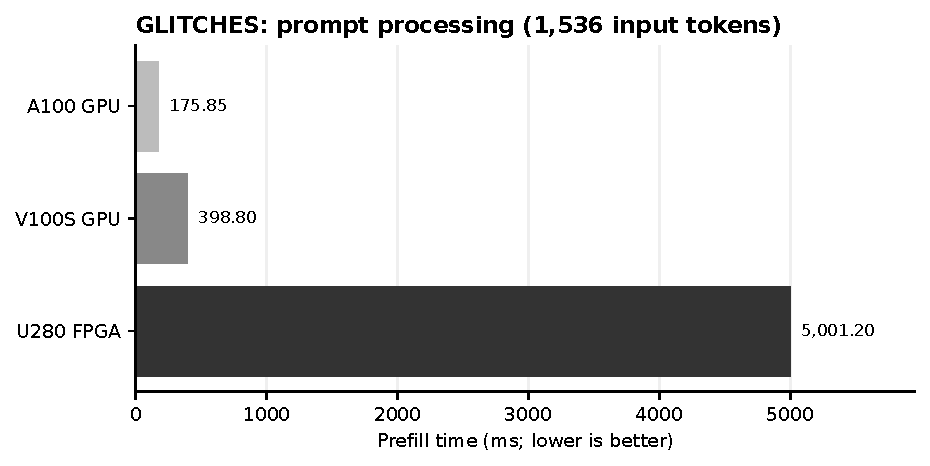
\includegraphics[width=\columnwidth]{figures/fig1_prefill_latency.pdf}
\caption{Reported GLITCHES prefill latency for a 1,536-token input (Table I in \cite{yang2024glitches}); lower is better. The GPU and FPGA use different numeric precision.}
\label{fig:prefill}
\end{figure}
\begin{figure}[t]
\centering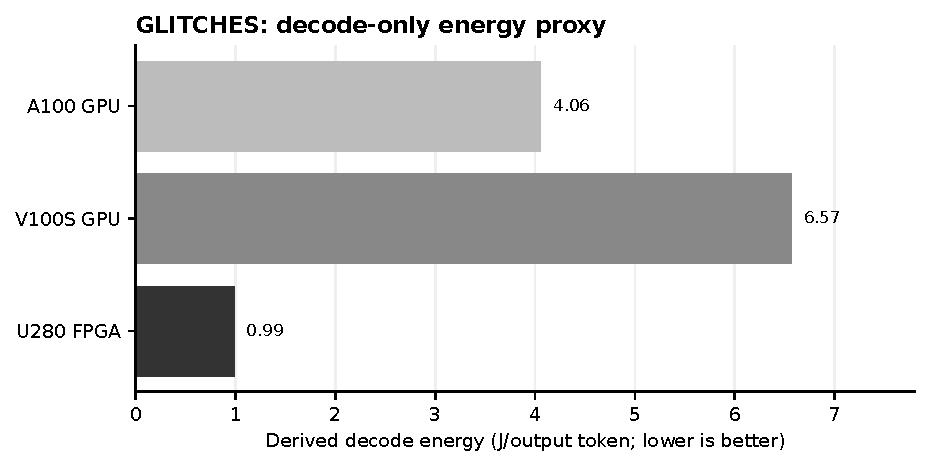
\includegraphics[width=\columnwidth]{figures/fig2_decode_energy.pdf}
\caption{Our derived decode-only energy per token from the reported power and decode time in GLITCHES Table I \cite{yang2024glitches}. Values exclude prefill and are not whole-system energy.}
\label{fig:energy}
\end{figure}
\subsection{Throughput and Energy Efficiency}
EdgeLLM implements a CPU--FPGA heterogeneous accelerator on the VCU128 using mixed FP16$\times$INT4 feed-forward computation, FP16$\times$FP16 attention computation, and structured sparsity \cite{huang2025edgellm}. For its evaluated sparse GLM-6B workload, the authors report a peak decoding rate of approximately 85.8 tokens/s and a normalized average FPGA power of 56.86~W. Their summary reports 1.91$\times$ throughput and 7.55$\times$ energy-efficiency improvements over the A100 GPU baseline. Table V of EdgeLLM~\cite{huang2025edgellm} also gives approximately 45 tokens/s and 0.2 tokens/s/W for A100 and 85.8 tokens/s and 1.51 tokens/s/W for EdgeLLM. These findings demonstrate the potential of FPGA acceleration under the evaluated configurations; however, performance advantages may vary with the model, hardware platform, and inference workload. For Qwen-7B, Table V of EdgeLLM~\cite{huang2025edgellm} reports 69.4 tokens/s and 1.23 tokens/s/W on the FPGA; the GLM-6B row is 85.8 tokens/s and 1.51 tokens/s/W. The approximately 75\% FPGA HBM bandwidth utilization is compared with approximately 30\% for the A100 in that table \cite{huang2025edgellm}.

\begin{figure}[t]
\centering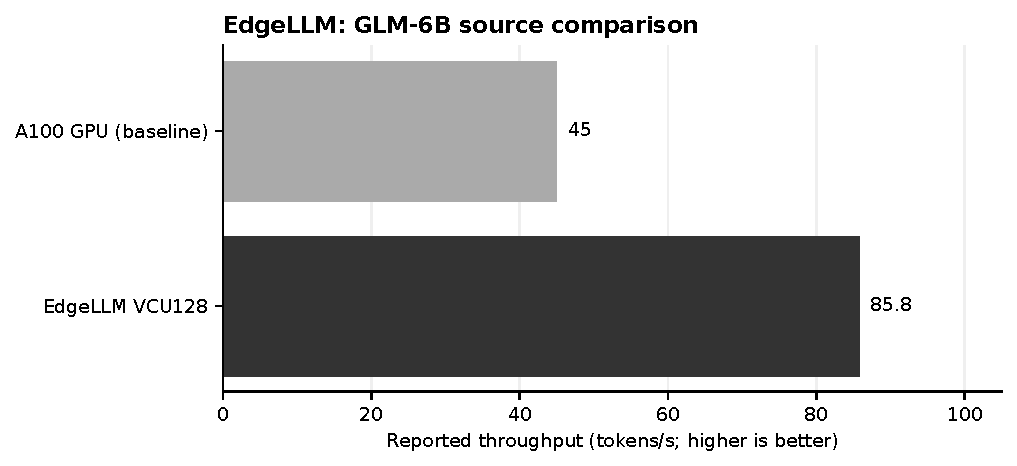
\includegraphics[width=\columnwidth]{figures/fig4_edgellm_throughput.pdf}
\caption{Source-reported throughput of the VCU128 and A100 configurations in EdgeLLM Table V \cite{huang2025edgellm}; comparison conditions and optimizations differ.}
\label{fig:edgellm}
\end{figure}
This result connects directly to the DDR/HBM tradeoff described in Section~III and the decode-memory bottleneck introduced in Section~II. Memory bandwidth materially changes the result even for the same accelerator. EdgeLLM reports a decode throughput of 51.42 tokens/s with HBM but 14.11 tokens/s with a DDR-based configuration for its 128-token evaluation; the associated prompt-processing rate falls from 0.51 to 0.24 tokens/s in the same source table \cite{huang2025edgellm}. This corresponds to a factor of $51.42/14.11\simeq 3.64$ in decode rate. Hence the memory hierarchy, not merely the number of arithmetic processing elements, is a major determinant of observed performance. However, the two configurations have different memory systems; this result should not be presented as an isolated measurement of bandwidth alone.

Hummingbird extends the discussion to smaller FPGA systems \cite{li2025hummingbird}. For 4-bit-weight LLaMA3-8B (with an 8-bit KV cache), it reports 4.8 tokens/s on KV260 and 8.6 tokens/s on ZCU104, with respective bandwidth efficiencies of about 94\% and 93\%. These throughput figures are reported for a 32-token prefill and 32-token decode benchmark, not at the maximum supported context length. The source lists memory bandwidths of 19.2 and 34.1~GB/s, so high \emph{fractional} utilization still corresponds to relatively limited absolute bytes/s compared with data-center devices. The authors also implement Hummingbird on an Alveo U250, reporting 19.4 tokens/s at 76.8~GB/s available bandwidth (Table V in the original Hummingbird paper). Table VI of Hummingbird~\cite{li2025hummingbird} lists 15 tokens/s for Jetson Orin Nano and 40 tokens/s for Jetson Orin AGX, with corresponding normalized power-efficiency figures of 1.0 and 0.66, compared with 1.44 and 1.39 for KV260 and ZCU104. Thus, the listed Jetson systems offer greater absolute token throughput, while the authors' normalized metric favors the FPGA designs. Its normalized power-efficiency measure is normalized performance divided by power, \emph{not} directly joules per token; Hummingbird reports the KV260 and ZCU104 device power as 3.81 and 7.09~W, respectively, as summarized in Table~\ref{tab:embedded}. These are not matched-bandwidth or necessarily matched-system-power experiments, and the Jetson results originate from a benchmark cited by Hummingbird \cite{li2025hummingbird}.

\begin{figure}[t]
\centering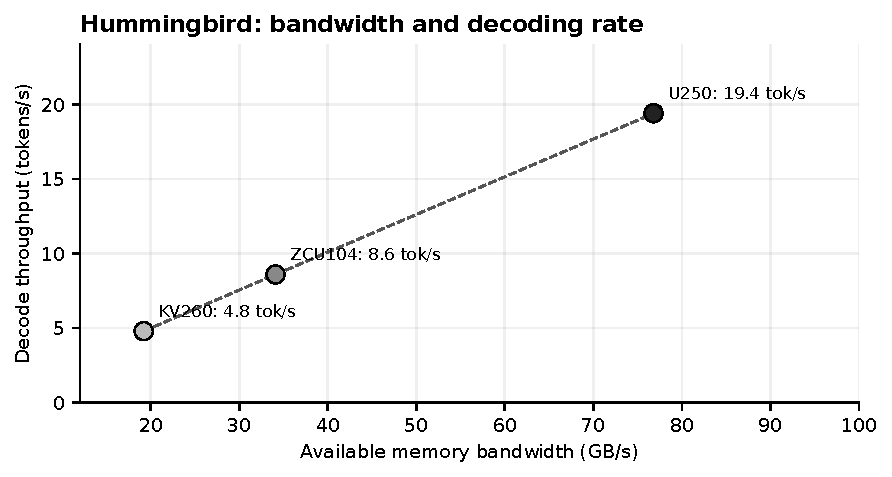
\includegraphics[width=\columnwidth]{figures/fig3_bandwidth_throughput.pdf}
\caption{Bandwidth and token generation rate reported for three Hummingbird FPGA boards (Table V in \cite{li2025hummingbird}); points do not constitute a controlled bandwidth-only experiment.}
\label{fig:bandwidth}
\end{figure}
\subsection{Architectural Tradeoffs and Scope of Evidence}
Section~III explains how systolic processing elements and pipelined offload paths can accelerate matrix operations. However, a design that performs well on matrix kernels may still suffer from sequential decoding or host--device transfers. The hardware--software co-design study on an Alveo U55 reports prompt-stage processing rates of 33.29 tokens/s (CPU-only), 71.58 tokens/s (first FPGA offload), and 124.0 tokens/s (larger FPGA offload) on INT8 TinyStories-15M \cite{chang2025codesign}. However, its decode rates are 10.9, 3.64, and 5.15 tokens/s, respectively. For the paper's 32 prompt tokens and 88 generated tokens, its end-to-end reported average throughput (Overall 1) is 13.28 tokens/s for software alone but only 4.87 and 6.92 tokens/s for the two full-offload variants. Keeping decoding on the CPU instead (Overall 2) raises the latter to 14.09 and 14.44 tokens/s. This reversal illustrates that a matrix-multiplication systolic array optimized for prompt processing may underutilize hardware during single-token decoding, particularly with PCIe transfers and offload overhead. In an equal 4,096-multiplier architectural comparison, the authors calculate a reduction in 64$\times$64 matrix-multiplication execution from 190 to 120 cycles using their systolic-array cycle model (Table I). Their analytical flip-flop \emph{storage-bit count} decreases from 194,560 to 45,056, while the reported I/O-channel requirement rises from 192 to 384 (Tables I--II). These architectural estimates should not be mistaken for separately measured post-implementation flip-flop counts or end-to-end latency. The study does not measure a GPU comparator; the prompt-only gains should not be reported as FPGA--GPU speedups.

Similarly, the layer-versus-spatial accelerator study reports speedups of 1.37$\times$ to 10.98$\times$ against two AMD EPYC CPUs for selected LLaMA2-7B operations \cite{prieto2024comparative}. The reported FPGA spatial design reduces the study's device-resource occupancy estimate from 33\% for the layer accelerator to 10\%, with DSPs falling from 4,036 to 1,277, LUTs from 411,098 to 99,290, and flip-flops from 1,143,511 to 238,519, while BRAM rises from 90 to 150 (Table I). Its optimized spatial FPGA architecture still trails the measured GPU in the cited 4096$\times$4096$\times$1 case, where the GPU is reported as 1.66$\times$ faster. The paper also notes that its operation-level FPGA timing can differ from end-to-end inference once data movement and orchestration are included. Its evidence therefore supports architectural tradeoff analysis rather than a general claim of FPGA superiority for complete LLM serving.

\par\noindent\textit{Embedded constraints, offloading, and the power--speed tradeoff.}\\ 
A key distinction is between \emph{bandwidth utilization} and \emph{absolute memory bandwidth}. Hummingbird obtains 93--94\% utilization of the DDR bandwidth available to its embedded systems, yet generates only 4.8--8.6 tokens/s on 8B-class models; the comparison cloud-class U250 implementation produces 19.4 tokens/s with 76.8~GB/s of bandwidth \cite{li2025hummingbird}. Its embedded devices also have smaller compute and memory budgets. Thus, even near-saturation of a small memory interface can leave token throughput below that of platforms with much larger absolute bandwidth. Table~\ref{tab:embedded} collects source-reported configurations; the values are not matched full-system GPU-versus-FPGA benchmarks.

\begin{table}[t]
\caption{Selected Hummingbird configurations for quantized LLaMA3-8B (Table V in the original Hummingbird study; reported device-level figures) \cite{li2025hummingbird}.}
\label{tab:embedded}
\centering\footnotesize
\begin{tabular}{lrrrr}
\hline
FPGA & BW (GB/s) & Decode (tok/s) & BW util. & Power (W)\\ \hline
KV260 & 19.2 & 4.8 & 94\% & 3.81\\
ZCU104 & 34.1 & 8.6 & 93\% & 7.09\\
U250 & 76.8 & 19.4 & 91\% & 14.61\\ \hline
\end{tabular}
\end{table}

As shown by Fig.~\ref{fig:bandwidth}, greater available bandwidth accompanies higher reported token throughput across the three FPGA boards, but their other hardware resources also differ. This observation links back to the KV-cache storage model in Section~II: high bandwidth utilization cannot compensate for a small absolute bandwidth or insufficient storage. Memory \emph{capacity} is a separate constraint. For its 4-GB embedded configurations, Hummingbird offloads the relatively large, FP16 embedding table to external flash, fetching only the needed token embedding when it is used; this frees faster main memory for quantized model weights and the KV cache. The authors combine this choice with grouped-query attention (GQA), which shares key/value heads across multiple query heads and reduces KV-cache storage compared with ordinary multi-head attention. Their LLaMA3-8B design supports a 4,096-token context, compared with the 1,024-token context cited for an earlier embedded \emph{different-model} LLaMA2-7B baseline; the reported 4.8/8.6 tokens/s rates, however, come from the 32:32-token benchmark \cite{li2025hummingbird}. Offloading is therefore a \emph{capacity-enabling} technique, not proof that slow external flash speeds up every memory access: it is favorable when the infrequently requested embeddings can be fetched without dominating per-token latency. This is distinct from streaming \emph{all} weights from flash; the latter configuration was not evaluated in the cited Hummingbird results.

Energy and responsiveness must likewise be evaluated together. Table I of GLITCHES~\cite{yang2024glitches} shows that the U280 uses 46.0~W and 21.50~ms/decode-token against 167.3~W and 24.26~ms/token for A100 under the paper's \emph{different-precision} conditions, but the U280 baseline's 5,001.20-ms prefill is far slower than A100's 175.85~ms \cite{yang2024glitches}. EdgeLLM's sparse, mixed-precision VCU128 obtains a favorable reported tokens/s/W ratio against A100, whereas Hummingbird's embedded FPGA systems sacrifice absolute generation rate for smaller measured device power and higher normalized power efficiency under the authors' definitions \cite{huang2025edgellm,li2025hummingbird}. The layer/spatial study additionally reports lower power during the evaluated FPGA operations (27~W) than during the GPU operations (35~W), yet finds the GPU faster for the evaluated kernel; lower watts alone does not establish lower joules per useful output \cite{prieto2024comparative}. Those kernel-power values cannot be interpreted as complete server power.

\subsection{Discussion and Implications}
The evidence can now be traced through the team's argument: Section~II identifies the computational and memory bottlenecks; Section~III proposes efficient processing, data reuse, low precision, and memory organization as solutions; this section quantifies the performance tradeoffs observed in published systems. Taken together, these published results inform four practical questions: embedded throughput is constrained by absolute memory and compute resources even with excellent bandwidth utilization; decode is sensitive to repeated weight/KV traffic; selective embedding offload and GQA can increase feasible model/context capacity; and lower device power may trade against prefill latency or absolute tokens/s. Across the five sources, FPGA competitiveness is strongest where (i) low-batch decoding is constrained by memory traffic rather than peak arithmetic throughput, (ii) reduced precision and carefully structured dataflow enable high effective bandwidth utilization, and (iii) a low-power deployment target justifies a specialized implementation \cite{huang2025edgellm,yang2024glitches,li2025hummingbird}. GPUs retain clear advantages for highly parallel prefill in the GLITCHES measurements, while hybrid GPU--FPGA processing can exploit the different computational profiles of the two inference phases \cite{yang2024glitches}. PCIe transfer, quantization overhead, differences in tested models, and inconsistent power accounting remain obstacles to direct cross-study ranking \cite{yang2024glitches,chang2025codesign,prieto2024comparative}.

Consequently, the evidence does not support the blanket statement that FPGAs are faster or more energy-efficient than GPUs for all LLM inference. It supports the narrower conclusion that appropriately optimized FPGA architectures can achieve competitive low-batch decoding and favorable reported energy-per-token figures under specified models, precisions, memory systems, and power boundaries. A definitive comparison would require the same model and quality target, matched prompt/decode workloads and batch sizes, measured device-and-host power, and explicit reporting of time to first token, time per output token, aggregate throughput, and joules per generated token. These five studies do not provide a single matched experiment satisfying all such conditions; cross-paper rankings of J/token would therefore be misleading. The Nexys A7 student-scale Transformer proposed in Section~III is a separate implementation objective, not an experimental reproduction of these published LLM benchmarks; its measured results must only be added after hardware verification.
